% Arquivo LaTeX de exemplo de dissertação/tese a ser apresentada à CPG do IME-USP
%
% Criação: Jesús P. Mena-Chalco
% Revisão: Fabio Kon e Paulo Feofiloff
% Adaptação para UTF8, biblatex e outras melhorias: Nelson Lago
%
% Except where otherwise indicated, these files are distributed under
% the MIT Licence. The example text, which includes the tutorial and
% examples as well as the explanatory comments in the source, are
% available under the Creative Commons Attribution International
% Licence, v4.0 (CC-BY 4.0) - https://creativecommons.org/licenses/by/4.0/


%%%%%%%%%%%%%%%%%%%%%%%%%%%%%%%%%%%%%%%%%%%%%%%%%%%%%%%%%%%%%%%%%%%%%%%%%%%%%%%%
%%%%%%%%%%%%%%%%%%%%%%%%%%%%%%% PREÂMBULO LaTeX %%%%%%%%%%%%%%%%%%%%%%%%%%%%%%%%
%%%%%%%%%%%%%%%%%%%%%%%%%%%%%%%%%%%%%%%%%%%%%%%%%%%%%%%%%%%%%%%%%%%%%%%%%%%%%%%%

% A opção twoside (frente-e-verso) significa que a aparência das páginas pares
% e ímpares pode ser diferente. Por exemplo, as margens podem ser diferentes ou
% os números de página podem aparecer à direita ou à esquerda alternadamente.
% Mas nada impede que você crie um documento "só frente" e, ao imprimir, faça
% a impressão frente-e-verso.
%
% Aqui também definimos a língua padrão do documento (a última da lista) e
% línguas adicionais. Para teses do IME, no mínimo português e inglês são
% obrigatórios, porque independentemente da língua principal do texto é
% preciso fornecer o resumo nessas duas línguas. LaTeX aceita alguns nomes
% diferentes para a língua portuguesa; dentre as opções, prefira sempre
% "brazilian" para português brasileiro e "portuguese" para português europeu.
%\documentclass[a4paper,12pt,twoside,brazilian,english]{book}
\documentclass[a4paper,12pt,twoside,english,brazilian]{book}

% O preâmbulo de um documento LaTeX pode ser razoavelmente longo. Neste
% modelo, optamos por reduzi-lo, colocando praticamente tudo do preâmbulo
% nas packages "imegoodies" e "imelooks".
%
% imegoodies carrega diversas packages muito úteis e populares (algumas
% são praticamente obrigatórias, como amsmath, babel, array etc.). É
% uma boa ideia usá-la com outros documentos também. Ela inclui vários
% comentários explicativos e dicas de uso; não tenha medo de alterá-la
% conforme a necessidade.
%
% imelooks carrega algumas packages e configurações que definem a
% aparência do documento; você também pode querer usá-la (ou partes
% dela) com outros documentos para obter as mesmas fontes, margens
% etc. Tal como "imegoodies", pode valer a pena ler os comentários
% e fazer modificações nessa package. Com a opção "thesis", imelooks
% também define os comandos para capa, folha de rosto etc.
\usepackage{imegoodies}
\usepackage[thesis]{imelooks}

%\nocolorlinks % para impressão em P&B

% Diretórios onde estão as figuras; com isso, não é necessário (mas
% é permitido) colocar o caminho completo em \includegraphics. Note
% que a extensão nunca é necessária (mas é permitida), ou seja, o
% resultado é o mesmo com "\includegraphics{figuras/foto.jpeg}",
% "\includegraphics{foto.jpeg}", "\includegraphics{figuras/foto}"
% ou "\includegraphics{foto}".
\graphicspath{{figuras/},{fig/},{logos/},{img/},{images/},{imagens/}}

% Comandos rápidos para mudar de língua:
% \en -> muda para o inglês
% \br -> muda para o português
% \texten{blah} -> o texto "blah" é em inglês
% \textbr{blah} -> o texto "blah" é em português
\babeltags{br = brazilian, en = english}


%%%%%%%%%%%%%%%%%%%%%%%%%%%%%%%%%%%%%%%%%%%%%%%%%%%%%%%%%%%%%%%%%%%%%%%%%%%%%%%%
%%%%%%%%%%%%%%%%%%%%%%%%%%%%%%%%%% METADADOS %%%%%%%%%%%%%%%%%%%%%%%%%%%%%%%%%%%
%%%%%%%%%%%%%%%%%%%%%%%%%%%%%%%%%%%%%%%%%%%%%%%%%%%%%%%%%%%%%%%%%%%%%%%%%%%%%%%%

% O arquivo com os dados bibliográficos para biblatex; você pode usar
% este comando mais de uma vez para acrescentar múltiplos arquivos
\addbibresource{bibliografia.bib}

% Este comando permite acrescentar itens à lista de referências sem incluir
% uma referência de fato no texto (pode ser usado em qualquer lugar do texto)
%\nocite{bronevetsky02,schmidt03:MSc, FSF:GNU-GPL, CORBA:spec, MenaChalco08}
% Com este comando, todos os itens do arquivo .bib são incluídos na lista
% de referências
%\nocite{*}

% É possível definir como determinadas palavras podem (ou não) ser
% hifenizadas; no entanto, a hifenização automática geralmente funciona bem
\babelhyphenation{documentclass latexmk soft-ware clsguide} % todas as línguas
\babelhyphenation[brazilian]{Fu-la-no}
\babelhyphenation[english]{what-ever}

% Estes comandos definem o título e autoria do trabalho e devem sempre ser
% definidos, pois além de serem utilizados para criar a capa, também são
% armazenados nos metadados do PDF. O subtítulo é opcional.
\title{Desenvolvimento de um sistema descentralizado de envio de mensagens}[Uma análise das dificuldades e limitações de sistemas descentralizados]
\translatedtitle{Development of a descentralized messaging system}[An analysis of the difficulties and limitations of descentralized systems]

\author[masc]{João Renner Rudge}

% \def\profa{Prof\kern.02em.\kern-.07emª\kern.07em}
% \def\dra{Dr\kern-.04em.\kern-.11emª\kern.07em}

% Para TCCs, este comando define o supervisor
\orientador[masc]{Prof. Dr. Daniel Macêdo Batista}

% Se não houver, remova; se houver mais de um, basta
% repetir o comando quantas vezes forem necessárias
% \coorientador{Prof. Dr. Ciclano de Tal}
% \coorientador[fem]{\profa{} \dra{} Beltrana de Tal}

% \banca{
%   \profa{} \dra{} Fulana de Tal (orientadora) -- IME-USP [sem ponto final],
%   % Em inglês, não há o "ª"
%   %Prof. Dr. Fulana de Tal (advisor) -- IME-USP [sem ponto final],
%   Prof. Dr. Ciclano de Tal -- IME-USP [sem ponto final],
%   \profa{} \dra{} Convidada de Tal -- IMPA [sem ponto final],
% }

% A página de rosto da versão para depósito (ou seja, a versão final
% antes da defesa) deve ser diferente da página de rosto da versão
% definitiva (ou seja, a versão final após a incorporação das sugestões
% da banca).
\tipotese{
  %mestrado,
  %doutorado,
  tcc,
  %definitiva, % É a versão para defesa ou a versão definitiva?
  %quali, % É qualificação?
  programa={Ciência da Computação},
}

\defesa{
  local={São Paulo},
  data=2024-04-03, % YYYY-MM-DD
}

% Se não houve bolsa, remova
%
% Norma sobre agradecimento por auxílios da FAPESP:
% https://fapesp.br/11789/referencia-ao-apoio-da-fapesp-em-todas-as-formas-de-divulgacao
%
% Norma sobre agradecimento por auxílios da CAPES (Portaria 206,
% de 4 de Setembro de 2018):
% https://www.in.gov.br/materia/-/asset_publisher/Kujrw0TZC2Mb/content/id/39729251/do1-2018-09-05-portaria-n-206-de-4-de-setembro-de-2018-39729135
%
%\apoio{O presente trabalho foi realizado com apoio da Coordenação
%      de Aperfeiçoamento\\ de Pessoal de Nível Superior -- Brasil
%      (CAPES) -- Código de Financiamento 001} % o código é sempre 001
%
%\apoio{This study was financed in part by the Coordenação de
%      Aperfeiçoamento\\ de Pessoal de Nível Superior -- Brasil
%      (CAPES) -- Finance Code 001} % o código é sempre 001
%
%\apoio{Durante o desenvolvimento deste trabalho, o autor recebeu\\
%      auxílio financeiro da FAPESP -- processo nº aaaa/nnnnn-d}
%
%\apoio{During the development if this work, the author received\\
%      financial support from FAPESP -- grant \#aaaa/nnnnn-d}
% \apoio{Durante o desenvolvimento deste trabalho o autor
%        recebeu auxílio financeiro da XXXX}

% A licença do seu trabalho. Use CC-BY, CC-BY-NC, CC-BY-ND, CC-BY-SA,
% CC-BY-NC-SA ou CC-BY-NC-ND para escolher a licença Creative Commons
% correspondente (o sistema insere automaticamente o texto da licença).
% Se quiser estabelecer regras diferentes para o uso de seu trabalho,
% converse com seu orientador e coloque o texto da licença aqui, mas
% observe que apenas TCCs sob alguma licença Creative Commons serão
% acrescentados ao BDTA. Se você tem alguma intenção de publicar o
% trabalho comercialmente no futuro, sugerimos a licença CC-BY-NC-ND.
%
%\direitos{CC-BY-NC-ND}
%
%\direitos{Autorizo a reprodução e divulgação total ou parcial deste
%          trabalho, por qualquer meio convencional ou eletrônico,
%          para fins de estudo e pesquisa, desde que citada a fonte.}
%
%\direitos{I authorize the complete or partial reproduction and disclosure
%          of this work by any conventional or electronic means for study
%          and research purposes, provided that the source is acknowledged.}
%
\direitos{CC-BY}

% Para gerar a ficha catalográfica, acesse https://fc.ime.usp.br/,
% preencha o formulário e escolha a opção "Gerar Código LaTeX".
% Basta copiar e colar o resultado aqui.
\fichacatalografica{}

\usepackage{xcolor}
\definecolor{amber}{rgb}{1.0, 0.49, 0.0}
\definecolor{cadmiumgreen}{rgb}{0.0, 0.42, 0.24}

\usepackage{amsthm}
\usepackage{tikz}
\usepackage{tcolorbox}

\newtheoremstyle{styleth}%
{3pt}% Space above
{3pt}% Space below 
{}% Body font
{}% Indent amount
{\bfseries\color{black}}% Theorem head font
{}% Punctuation after theorem head
{.5em}% Space after theorem head
{}% Theorem head spec (can be left empty, meaning ‘normal’)
\theoremstyle{styleth}
\newtheorem{defin}{Definição}

\newcommand{\statetheoremsolid}[2][\textwidth]{
  \par\noindent\tikzstyle{mybox} = [draw=black,fill=white,
   thick,rectangle,rounded corners,inner sep=6pt]
  \begin{tikzpicture}
    \node [mybox] (box){%
    \begin{minipage}{#1}{#2}\end{minipage}
   };
  \end{tikzpicture}
}

%%%%%%%%%%%%%%%%%%%%%%%%%%%%%%%%%%%%%%%%%%%%%%%%%%%%%%%%%%%%%%%%%%%%%%%%%%%%%%%%
%%%%%%%%%%%%%%%%%%%%%%% AQUI COMEÇA O CONTEÚDO DE FATO %%%%%%%%%%%%%%%%%%%%%%%%%
%%%%%%%%%%%%%%%%%%%%%%%%%%%%%%%%%%%%%%%%%%%%%%%%%%%%%%%%%%%%%%%%%%%%%%%%%%%%%%%%

\begin{document}

%%%%%%%%%%%%%%%%%%%%%%%%%%% CAPA E PÁGINAS INICIAIS %%%%%%%%%%%%%%%%%%%%%%%%%%%%

% Aqui começa o conteúdo inicial que aparece antes do capítulo 1, ou seja,
% página de rosto, resumo, sumário etc. O comando frontmatter faz números
% de página aparecem em algarismos romanos ao invés de arábicos e
% desabilita a contagem de capítulos.
\frontmatter

\pagestyle{plain}

\onehalfspacing % Espaçamento 1,5 na capa e páginas iniciais

\maketitle % capa e folha de rosto

%%%%%%%%%%%%%%%% DEDICATÓRIA, AGRADECIMENTOS, RESUMO/ABSTRACT %%%%%%%%%%%%%%%%%%

% \begin{dedicatoria}
% Esta seção é opcional e fica numa página separada; ela pode ser usada para
% uma dedicatória ou epígrafe.
% \end{dedicatoria}

% Reinicia o contador de páginas (a próxima página recebe o número "i") para
% que a página da dedicatória não seja contada.
\pagenumbering{roman}

% Agradecimentos:
% Se o candidato não quer fazer agradecimentos, deve simplesmente eliminar
% esta página. A epígrafe, obviamente, é opcional; é possível colocar
% epígrafes em todos os capítulos. O comando "\chapter*" faz esta seção
% não ser incluída no sumário.
\chapter*{Agradecimentos}
\epigrafe{Lets see what happens.}{Unnamed fictional character from Randall Munroe's \textit{what if?}}

À minha família, por sempre me apoiar nos meus estudos, me educar, me permitir
chegar onde estou hoje; ao computador do escritório da minha
mãe, por cativar minha curiosidade e me ensinar uma infinitude de coisas ao
longo da minha infância; aos meus amigos, por sempre estarem do meu lado, 
fazendo companhia, me dando algo para fazer todo dia.

%!TeX root=../tese.tex
%("dica" para o editor de texto: este arquivo é parte de um documento maior)
% para saber mais: https://tex.stackexchange.com/q/78101

% As palavras-chave são obrigatórias, em português e em inglês, e devem ser
% definidas antes do resumo/abstract. Acrescente quantas forem necessárias.
\palavraschave{Palavra-chave1, Palavra-chave2, Palavra-chave3}

\keywords{Keyword1,Keyword2,Keyword3}

% O resumo é obrigatório, em português e inglês. Estes comandos também
% geram automaticamente a referência para o próprio documento, conforme
% as normas sugeridas da USP.
\resumo{
Elemento obrigatório, constituído de uma sequência de frases concisas e
objetivas, em forma de texto. Deve apresentar os objetivos, métodos empregados,
resultados e conclusões. O resumo deve ser redigido em parágrafo único, conter
no máximo 500 palavras e ser seguido dos termos representativos do conteúdo do
trabalho (palavras-chave). Deve ser precedido da referência do documento.
Texto texto texto texto texto texto texto texto texto texto texto texto texto
texto texto texto texto texto texto texto texto texto texto texto texto texto
texto texto texto texto texto texto texto texto texto texto texto texto texto
texto texto texto texto texto texto texto texto texto texto texto texto texto
texto texto texto texto texto texto texto texto texto texto texto texto texto
texto texto texto texto texto texto texto texto.
Texto texto texto texto texto texto texto texto texto texto texto texto texto
texto texto texto texto texto texto texto texto texto texto texto texto texto
texto texto texto texto texto texto texto texto texto texto texto texto texto
texto texto texto texto texto texto texto texto texto texto texto texto texto
texto texto.
}

\abstract{
Elemento obrigatório, elaborado com as mesmas características do resumo em
língua portuguesa. De acordo com o Regimento da Pós-Graduação da USP (Artigo
99), deve ser redigido em inglês para fins de divulgação. É uma boa ideia usar
o sítio \url{www.grammarly.com} na preparação de textos em inglês.
Text text text text text text text text text text text text text text text text
text text text text text text text text text text text text text text text text
text text text text text text text text text text text text text text text text
text text text text text text text text text text text text.
Text text text text text text text text text text text text text text text text
text text text text text text text text text text text text text text text text
text text text.
}



%%%%%%%%%%%%%%%%%%%%%%%%%%% LISTAS DE FIGURAS ETC. %%%%%%%%%%%%%%%%%%%%%%%%%%%%%

% Como as listas que se seguem podem não incluir uma quebra de página
% obrigatória, inserimos uma quebra manualmente aqui.
\cleardoublepage

% Todas as listas são opcionais; Usando "\chapter*" elas não são incluídas
% no sumário. As listas geradas automaticamente também não são incluídas por
% conta das opções "notlot" e "notlof" que usamos para a package tocbibind.

% Normalmente, "\chapter*" faz o novo capítulo iniciar em uma nova página, e as
% listas geradas automaticamente também por padrão ficam em páginas separadas.
% Como cada uma destas listas é muito curta, não faz muito sentido fazer isso
% aqui, então usamos este comando para desabilitar essas quebras de página.
% Se você preferir, comente as linhas com esse comando e des-comente as linhas
% sem ele para criar as listas em páginas separadas. Observe que você também
% pode inserir quebras de página manualmente (com \clearpage, veja o exemplo
% mais abaixo).
\newcommand\disablenewpage[1]{{\let\clearpage\par\let\cleardoublepage\par #1}}

% Nestas listas, é melhor usar "raggedbottom" (veja basics.tex). Colocamos
% a opção correspondente e as listas dentro de um grupo para ativar
% raggedbottom apenas temporariamente.
\bgroup
\raggedbottom

%%%%% Listas criadas manualmente

%\chapter*{Lista de abreviaturas}
\disablenewpage{\chapter*{Lista de abreviaturas}}

\begin{tabular}{rl}
  DNS & Sistema de Nomes de Domínio (\emph{Domain Name System})\\
  CDN & Rede de Distribuição de Conteúdo (\emph{Content Delivery Network})\\
  TLS & Segurança de Camada de Transporte (\emph{Transport Layer Security})\\
  P2P & \emph{Peer-to-Peer}\\
  TOR & \emph{The Onion Router}\\
  NAT & Tradução de Endereços de Rede (\emph{Network Address Translation})\\
  IRC & \emph{Internet Relay Chat}\\
  IoT & Internet das Coisas (\emph{Internet of Things})\\
  ITU-T & União Internacional de Telecomunicações - Setor de Padronização de Telecomunicações\\
  UPnP & \emph{Universal Plug and Play}\\
\end{tabular}

% Quebra de página manual
\clearpage

%%%%% Listas criadas automaticamente

% Você pode escolher se quer ou não permitir a quebra de página
%\listoffigures
\disablenewpage{\listoffigures}

% Você pode escolher se quer ou não permitir a quebra de página
%\listoftables
\disablenewpage{\listoftables}

% Sumário (obrigatório)
\tableofcontents

\egroup % Final de "raggedbottom"

% Referências indiretas ("x", veja "y") para o índice remissivo (opcionais,
% pois o índice é opcional). É comum colocar esses itens no final do documento,
% junto com o comando \printindex, mas em alguns casos isso torna necessário
% executar texindy (ou makeindex) mais de uma vez, então colocar aqui é melhor.
\index{Inglês|see{Língua estrangeira}}
\index{Figuras|see{Floats}}
\index{Tabelas|see{Floats}}
\index{Código-fonte|see{Floats}}
\index{Subcaptions|see{Subfiguras}}
\index{Sublegendas|see{Subfiguras}}
\index{Equações|see{Modo matemático}}
\index{Fórmulas|see{Modo matemático}}
\index{Rodapé, notas|see{Notas de rodapé}}
\index{Captions|see{Legendas}}
\index{Versão original|see{Tese/Dissertação, versões}}
\index{Versão corrigida|see{Tese/Dissertação, versões}}
\index{Palavras estrangeiras|see{Língua estrangeira}}
\index{Floats!Algoritmo|see{Floats, ordem}}


%%%%%%%%%%%%%%%%%%%%%%%%%%%%%%%% CAPÍTULOS %%%%%%%%%%%%%%%%%%%%%%%%%%%%%%%%%%%%%

% Aqui vai o conteúdo principal do trabalho, ou seja, os capítulos que compõem
% a dissertação/tese. O comando mainmatter reinicia a contagem de páginas,
% modifica a numeração para números arábicos e ativa a contagem de capítulos.
\mainmatter

\pagestyle{mainmatter}

% Espaçamento simples
\singlespacing

% A introdução não tem número de capítulo, então os cabeçalhos também não
\pagestyle{unnumberedchapter}
%!TeX root=../tese.tex
%("dica" para o editor de texto: este arquivo é parte de um documento maior)
% para saber mais: https://tex.stackexchange.com/q/78101

%% ------------------------------------------------------------------------- %%

% "\chapter" cria um capítulo com número e o coloca no sumário; "\chapter*"
% cria um capítulo sem número e não o coloca no sumário. A introdução não
% deve ser numerada, mas deve aparecer no sumário. Por conta disso, este
% modelo define o comando "\chapter**".
\chapter**{Introdução}
\label{cap:introducao}

\enlargethispage{.5\baselineskip}

A centralização progressiva da internet tem sido um fenômeno notável ao longo das últimas décadas, a despeito da sua arquitetura que é fundamentalmente descentralizada. Tal consolidação, causada por diversos fatores econômicos e sociais, fez com que o controle da rede tenha se concentrado cada vez mais nas mãos de um pequeno conjunto de empresas extremamente influentes. Tal situação levanta grandes preocupações sobre privacidade, segurança, e posse de dados pessoais, num cenário em que poucas aplicações amplamente utilizadas são de fato descentralizadas em arquitetura e governância.

Em uma análise mais detalhada, nota-se que esse fenômeno de centralização tem se apresentado em muitas componentes diferentes. Luciano Zembruzki junto de outros pesquisadores mostrou, por exemplo, como o mercado de hospedagem web se tornou extraordinariamente concentrado, e como apenas 10 provedores compunham quase toda a hospedagem dos domínios de topo de nível considerados em sua análise \cite{Zembruzki2022}. Por outro lado, Giovane Moura, Sebastian Castro, e outros em um estudo notaram que o Sistema de Nomes de Domínio tem sido modificado de maneira similar, apresentando "concentração notável" \cite{Moura2020}. Outros artigos relatam comportamentos similares em Content Delivery Networks (CDNs) e na propagação da versão mais recente do protocolo de segurança Transport Layer Security (TLS) 1.3 \cite{Vermeulen2023, Holz2020}. Assim, percebe-se que esse processo é muito difundido, e afeta multiplas facetas técnicas da internet moderna.

Por outro lado, mesmo numa perspectiva social e econômica a rede mundial de computadores tem passado por um constande processo de consolidação corporativa, fusões entre empresas, e uma presença cada vez maior de tecnologias proprietárias e ecossistemas fechados que evitam a migração dos usuários para serviços concorrentes. Tal processo é descrito em excelente detalhe por Ulrich Dolata no quinto capítulo do livro "Collectivity and Power on the Internet: A Social Perspective" \cite{UlrichDolata}.

Nesse sentido, a presença cada vez menor de protocolos de compartilhamento de arquivos e mensagens descentralizadas é um processo pelo menos parcialmente influenciado por entidades comerciais, uma vez que companhias tem diversas vantagens e incentivos para controlar e manejar cada vez mais dados de seus clientes, ao invés de delegá-los a um sistema autônomo. Além disso, sistemas abertos e controlados por seus usuários muitas vezes requerem um nível mais elevado de conhecimento técnico para serem utilizados, tornando-se menos preferíveis para o consumidor médio. É muito comum que soluções comerciais tenham mais suporte e sejam mais convenientes e simples de se utilizar, adquirindo assim mais clientes ao longo prazo. Assim, um sistema distribuido que consiga lidar com todos os aspectos técnicos da transmissão de mensagens de forma descentralizada pode ser uma solução preferível para um usuário que prefere não ter seus dados pessoais controlados por uma entidade com fins lucrativos. 

Nexte contexto, esta monografia tem como objetivo uma análise técnica das limitações de sistemas abertos de envio de mensagens, considerando aspectos como a arquitetura descentralizada, sincronicidade, confiabilidade na entrega de mensagens e resistência a atores mal-intencionados. Embora existam diversas implementações de protocolos descentralizados de código aberto, este trabalho não tem como objetivo criar um protocolo completamente abrangente que substitua todos os demais. Em vez disso, ele busca uma análise crítica e abrangente dessas soluções, destacando suas vantagens e limitações. Essa avaliação é fundamental para informar futuros estudos e o desenvolvimento de novos protocolos. Além disso, a criação de uma prova de conceito desempenha um papel essencial neste estudo, ao permitir a aplicação prática das ideias discutidas, demonstrando concretamente seus méritos e desafios.

\pagestyle{mainmatter}
%!TeX root=../tese.tex
%("dica" para o editor de texto: este arquivo é parte de um documento maior)
% para saber mais: https://tex.stackexchange.com/q/78101

\chapter{Definições importantes}

Antes de analisar implementações existentes de protocolos de envio de mensagens descentralizados, é importante definir alguns conceitos e características importantes para a compreensão do funcionamento desses protocolos. Este capitulo será dedicado a explicar importantes definições e características de protocolos de comunicação.

\section{Protocolos de comunicação}

Uma primeira distinção importante a ser feita é entre protocolos de comunicação centralizados e descentralizados. A partir dessas definições é possível definir melhor outros termos e conceitos relacionados a protocolos de comunicação.

\statetheoremsolid{
\begin{defin}
    Um \textbf{protocolo centralizado} de envio de mensagens é aquele em que suas comunicações passam por servidores controlados por uma única entidade ou organização. Nesse modelo, os servidores centrais gerenciam a transmissão e roteamento das mensagens. Em muitos casos essa entidade central também pode ser responsável pelo armazenamento e criptografia dos dados dos usuários. 
\end{defin}
}

Um protocolo com arquitetura centralizada permite um controle mais rigoroso sobre o fluxo de dados, o que facilita a implementação de funcionalidades como backups, moderação de conteúdo e integração com outros serviços. No entanto, essa centralização também implica riscos, como maior vulnerabilidade a falhas de segurança, falhas de serviço e questões relacionadas à privacidade, já que todos os dados dos usuários são concentrados em um único ponto. Além disso, a dependência de uma entidade centralizada pode levar a restrições de acesso e à censura, uma vez que o controle das comunicações está nas mãos de uma única organização.

Por outro lado, podemos definir um protocolo descentralizado como:

\statetheoremsolid{
\begin{defin}
    Um \textbf{protocolo descentralizado} de envio de mensagens é aquele em que as comunicações são distribuídas entre vários nós ou servidores, sem a necessidade de uma entidade central para gerenciar ou governar o fluxo de dados. Nesse modelo, os usuários podem se comunicar diretamente uns com os outros, sem depender de intermediários centralizados.
\end{defin}
}

Os protocolos descentralizados têm várias vantagens em relação aos centralizados, como maior resistência a falhas, maior privacidade e menor vulnerabilidade a censura. No entanto, eles também apresentam desafios, como a necessidade de garantir a integridade e a consistência dos dados em um ambiente distribuído e a necessidade de lidar com questões de escalabilidade e desempenho. Além disso, a ausência de uma entidade centralizada pode dificultar a implementação de certas funcionalidades, como backups, moderação de conteúdo e integração com outros serviços.

Uma vez que a transmissão de dados na rede passa por muitos computadores até chegar ao seu destino, é importante garantir que esses dados sejam transmitidos de forma segura e confiável. Uma maneira de fazer isso é através da criptografia. Podemos a definir como:

\statetheoremsolid{
\begin{defin}
    A \textbf{criptografia} é o processo de codificar informações de forma que apenas o destinatário pretendido possa decodificá-las. A criptografia é amplamente utilizada em protocolos de comunicação para garantir a confidencialidade, integridade e autenticidade dos dados transmitidos.
\end{defin}
}

Sistemas de comunicação modernos podem utilizar criptografia em passos discretos do processo de comunicação, ou no caminho completo de ponta a ponta. A criptografia de ponta a ponta é um método de criptografia em que os dados são criptografados no dispositivo do remetente e só podem ser descriptografados no dispositivo do destinatário. Isso garante que os dados permaneçam seguros, mesmo se forem roteados por uma entidade central, ou sejam transmitidos por uma rede não confiável.

Algumas outras definições importantes para discussões nesse capítulo incluem:

\section{Características de protocolos de comunicação}

Além das definições acima, existem várias características importantes que podem ser usadas para avaliar e comparar diferentes protocolos de envio de mensagens descentralizados. Algumas dessas características incluem:

\begin{itemize}
    \item \textbf{Privacidade de metadados:} Mesmo que a grande maioria dos protocolos modernos de comunicação garantam a privacidade do conteúdo das mensagens, muitos deles ainda coletam e armazenam metadados, como informações sobre quem enviou a mensagem, quando foi enviada e para quem foi enviada. Além disso, durante a sua transmissão, dados relacionados com os computadores de origem e destino, informações de interfaces de rede, endereços de IP podem ser coletadas por terceiros. Protocolos que garantem a privacidade de metadados são capazes de proteger essas informações e garantir que elas permaneçam privadas.
    
    \item \textbf{Escalabilidade:} A escalabilidade é a capacidade de um sistema de crescer e lidar com um aumento no número de usuários e mensagens sem comprometer o desempenho. Protocolos não escaláveis não conseguem lidar com um aumento da demanda mesmo com a adição de mais recursos.
    
    \item \textbf{Interoperabilidade:} A interoperabilidade é a capacidade de diferentes sistemas e protocolos de comunicação trabalharem juntos de forma eficiente e eficaz. Alguns protocolos analisados nesta monografia são mais versáteis e implementam uma série de padrões e especificações que permitem a comunicação com outros sistemas e protocolos.

    \item \textbf{Assincronicidade:} Protocolos assíncronos permitem que os usuários enviem mensagens sem depender da disponibilidade do destinatário. Esta funcionalidade geralmente depende de um sistema de armazenamento de mensagens, que pode ser centralizado ou não, que permite que as mensagens sejam entregues mesmo quando o destinatário não está online.
\end{itemize}

\section {Redes locais, NATs e firewalls}

A grande maioria de usuários da internet não possuem diretamente um endereço de IP público, que é um endereço único e globalmente acessível que identifica um dispositivo na internet. Em vez disso, eles estão conectados a uma rede local, que é uma rede privada em que múltiplos dispositivos compartilham um único endereço de IP público. O roteador é o dispositivo reponsável por gerenciar o tráfego de dados entre a rede local e a internet, redirecionando dados recebidos externamente para os dispositivos corretos na rede local. 

\section {Relays em protocolos de comunicação}

Um tipo de computador comumente utilizado em protocolos de comunicação descentralizados é o relay.

\statetheoremsolid{
\begin{defin}
    Um \textbf{relay} é um servidor intermediário que ajuda a encaminhar mensagens entre diferentes usuários em um protocolo de comunicação descentralizado. Os relays geralmente possuem arquitetura interna bem simples, apenas encaminhando mensagens entre usuários, sem armazenar ou processar dados.
\end{defin}
}

Relays são principalmente utilizados para contornar restrições de roteamento em redes que possuem camadas de Network Address Translation (NAT) ou firewalls, que podem impedir a comunicação direta entre dois usuários. Outras funcionalidades que eles podem prover incluem a capacidade de armazenar mensagens temporariamente, para que possam ser entregues mesmo quando o destinatário não está online, e a capacidade de diminuir os metadados que estão sendo transmitidos, uma vez que ele pode ocultar o endereço IP real do remetente e destinatário.

\section{The Onion Router (Tor)}

O Tor é uma rede de comunicação descentralizada que permite que os usuários naveguem na internet de forma anônima e segura. Ele é composto por uma rede de servidores de voluntários, chamados de relays, que se dispõe a redirecionar o tráfego de internet de forma anônima. Como estes voluntários são desconhecidos, o protocolo da rede é desenhado para minimizar a quantidade de informações que cada relay tem acesso, garantindo a privacidade dos usuários. Esta rede pode ser utilizada tanto para navegação em websites comuns da internet com mais privacidade, assim como para acessar serviços ocultos, que são sites que só podem ser acessados através da rede Tor.

\subsection{Acesso a sites comuns}

Quando um usuário acessa um site comum da internet através da rede Tor, a sua conexão é roteada através de três relays diferentes, chamados de entrada, intermediário e saída. Cada relay apenas tem acesso a informações sobre o relay anterior e o próximo, o que ajuda a limitar a quantidade de informações que cada relay tem acesso:

\begin{itemize}
    \item O relay de entrada sabe o endereço IP do usuário, mas não sabe o que ele está acessando.
    \item O relay intermediário não sabe nada sobre usuários e não pode ver o conteúdo transmitido.
    \item O relay de saída sabe que algum usuário da rede está acessando aquele serviço, mas não sabe quem é o usuário.
\end{itemize}

Um vídeo excelente publicado pela Universidade de Nottingham que entra em mais detalhes sobre a troca de chaves e a criptografia do protocolo Tor pode ser encontrado em \cite{computerphile}.

A utilização do protocolo Tor para acessar sites comuns da internet é conceitualmente similar a utilizar um serviço de Virtual Private Network (VPN). Ambos agem como um intermediário entre o usuário e o site acessado, escondendo o endereço IP real do usuário e protegendo a sua privacidade. No entanto, enquanto Tor é gratuito, mais anônimo e descentralizado, VPNs são pagas, centralizadas, mas geralmente possuem melhor desempenho.

\subsection{Acesso a serviços ocultos}

Além de permitir o acesso a sites comuns da internet de forma anônima, o Tor também suporta a criação e acesso a serviços ocultos, que são sites que só podem ser acessados através da rede Tor. Estes sites possuem um endereço especial, terminado em .onion, que é gerado a partir de uma chave pública do servidor. A utilização de serviços ocultos permite que os usuários hospedem sites de forma anônima e segura, sem precisarem de um firewall aberto e sem revelar a localização física do servidor.
%!TeX root=../tese.tex
%("dica" para o editor de texto: este arquivo é parte de um documento maior)
% para saber mais: https://tex.stackexchange.com/q/78101

\chapter{Implementações já existentes}

Este capítulo da monografia realizará a análise de implementações de código aberto já existentes de protocolos descentralizados de envio de mensagens. Essas implementações fornecem uma base para compreender os desafios práticos, as abordagens de arquitetura e as estratégias de mitigação de problemas que foram desenvolvidas e testadas pela comunidade. Os protocolos analisados foram selecionados por serem abertos, descentralizados, e por terem uma arquitetura de rede singular, sendo relevante para este estudo. Os protocolos analisados foram categorizados pela sua arquitetura de rede, e divididos em quatro grupos principais: federados, peer-to-peer com relays que usam tor, peer-to-peer com relays que não usam tor, e peer-to-peer sem relays.

Os protocolos analisados federados são:
\begin{itemize}
  \item \href{https://matrix.org/}{Matrix}
  \item \href{https://xmpp.org/}{XMPP}
  \item \href{https://datatracker.ietf.org/doc/html/rfc5321}{E-Mail}
\end{itemize}

Os protocolos analisados peer-to-peer com relays que não usam Tor são:
\begin{itemize}
  \item \href{https://simplex.chat/}{SimpleX}
  \item \href{https://datatracker.ietf.org/doc/html/rfc2810}{IRC}
  \item \href{https://lora-alliance.org/}{LoRaWan}
\end{itemize}

Os protocolos analisados peer-to-peer com relays que usam Tor são:
\begin{itemize}
  \item \href{https://cwtch.im/}{Cwtch}
  \item \href{https://ricochet.im/}{Ricochet}
  \item \href{https://briarproject.org/}{Briar}
\end{itemize}

Os protocolos analisados peer-to-peer sem relays são:
\begin{itemize}
  \item \href{https://scuttlebutt.nz/}{Secure Scuttlebutt}
  \item \href{https://tox.chat/}{Tox}
  \item \href{https://bitmessage.org/}{Bitmessage}
\end{itemize}

A análise de cada protocolo é focada na arquitetura de rede, e não considera em detalhes outras funcionalidades como chamadas de voz, videoconferência, ou compartilhamento de arquivos. A seguir, são apresentadas as análises dos protocolos selecionados.

\section{Protocolos Federados}

Na arquitetura federada de envio de mensagens, cada usuário escolhe um servidor para ser seu provedor de mensagens. Essa maquina será responsável por rotear todas as comunicações do usuário, e em alguns casos também armazenar suas mensagens. É importante que o usuário possa confiar no seu provedor de mensagens, uma vez que ele é um intermediário de todas as comunicações do usuário, que muitas vezes podem ser não criptografadas.

Caso um usuário queira se comunicar com outro usuário em um servidor diferente, os servidores precisam se comunicar entre si para rotear as mensagens. Como o servidor é responsável pelo recebimento e entrega das mensagens, os protocolos federados permitem o envio assíncrono de mensagens. Em geral, os endereços dos usuários nesses sistemas consistem em uma combinação de um nome de usuário com o endereço do servidor.

\begin{figure}
  \centering
  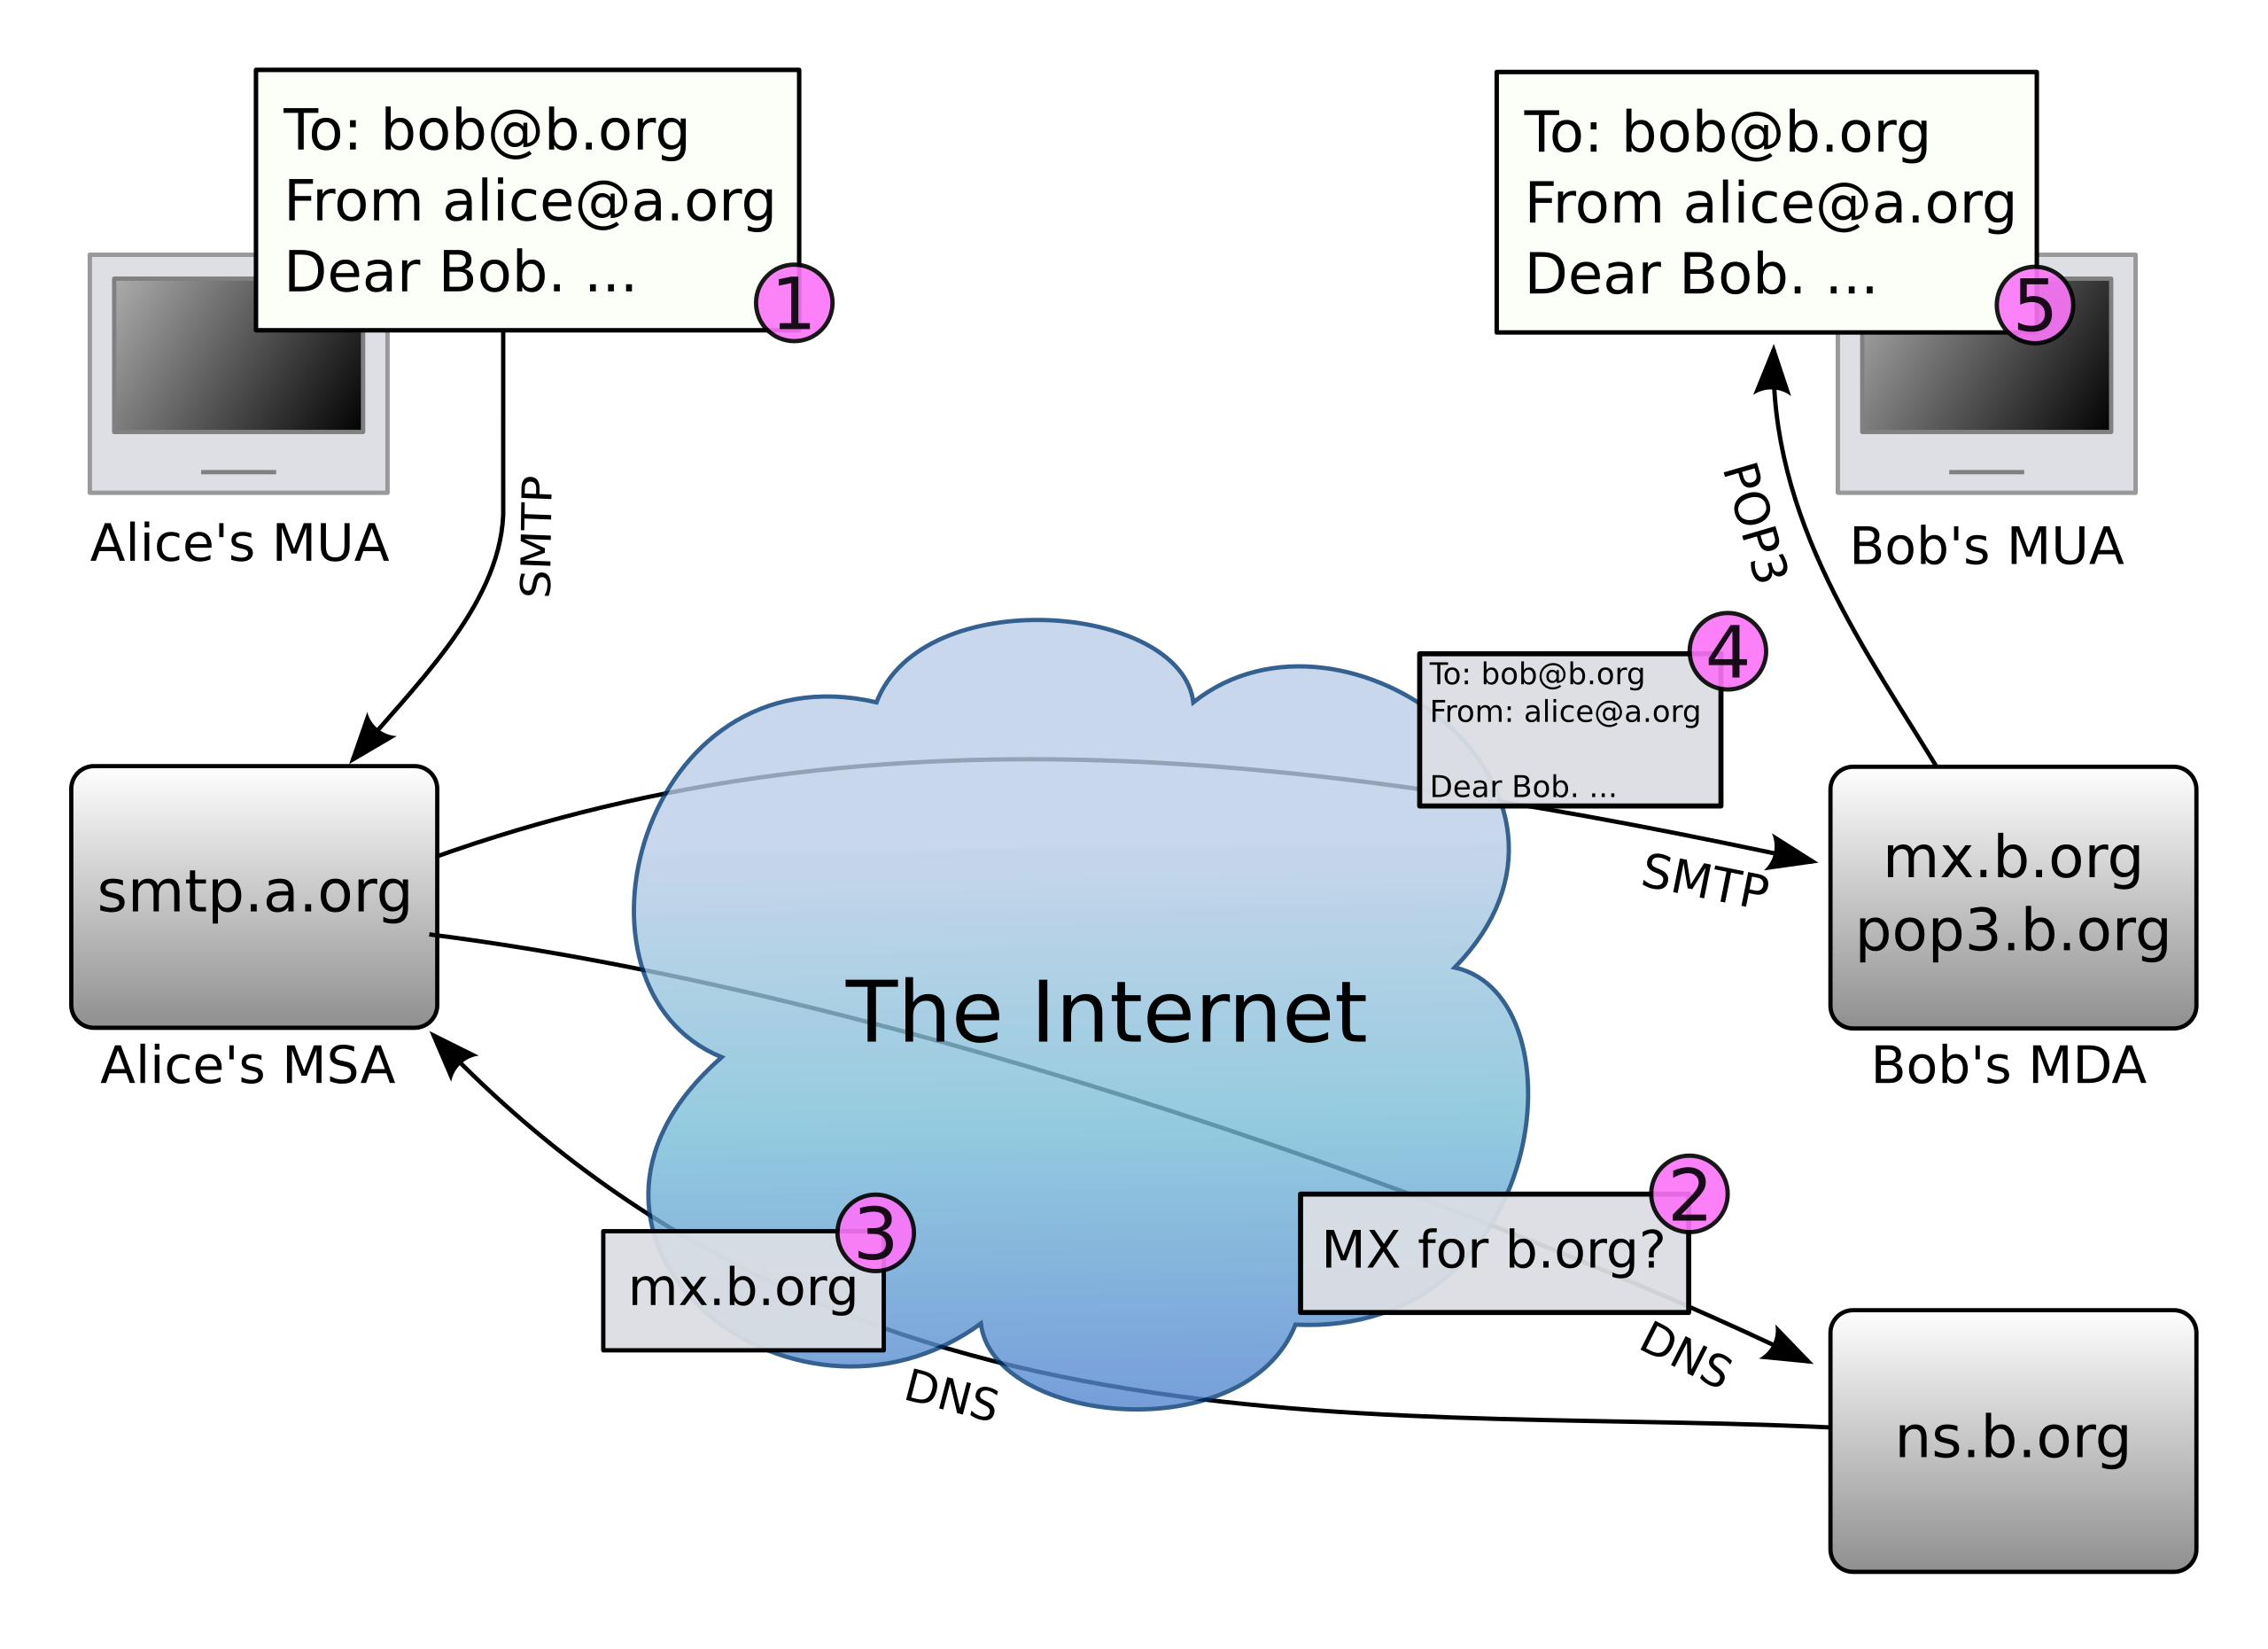
\includegraphics[width=0.5\textwidth]{federated-email}

  % remember to cite the source of the image
  \caption{Arquitetura do email, um protocolo federado. \cite{email-picture}}
\end{figure}

\subsection{E-Mail}

O e-mail (correio eletrônico) é um sistema de comunicação digital que permite o envio e recebimento de mensagens e arquivos entre usuários através de redes de computadores, utilizando protocolos como SMTP, POP3 e IMAP para a transmissão e armazenamento das mensagens. É amplamente utilizado para comunicação pessoal e profissional, sendo uma das formas mais comuns de troca de informações na Internet. \cite{rfc5321}

\begin{itemize}
  \item \textbf{Tipo de endereço}: usuário@servidor
  \item \textbf{Suporte a criptografia de ponta a ponta}: Sim
\end{itemize}

\subsection{Matrix}

O protocolo Matrix é um sistema de comunicação descentralizado e federado projetado para suportar mensagens instantâneas e colaboração em tempo real. Desenvolvido para ser uma solução aberta e interoperável, o Matrix visa fornecer uma infraestrutura robusta para comunicação em diversos contextos, desde chat e chamadas de voz até a troca de arquivos. \cite{matrixspec}

\begin{figure}
  \centering
  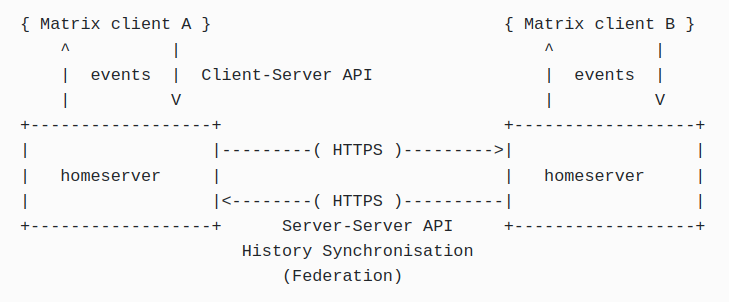
\includegraphics[width=0.5\textwidth]{matrix}

  % remember to cite the source of the image
  \caption{Arquitetura do protocolo Matrix \cite{matrixspec}}
\end{figure}

\begin{itemize}
  \item \textbf{Tipo de endereço}: @usuário:servidor
  \item \textbf{Suporte a criptografia de ponta a ponta}: Sim
\end{itemize}

\subsection{XMPP}

XMPP (Extensible Messaging and Presence Protocol) é um protocolo de comunicação em tempo real, baseado em XML, que permite a troca descentralizada e segura de mensagens, presença e dados estruturados entre clientes e servidores, suportando uma ampla variedade de funcionalidades, como chat, voz, vídeo e colaboração em grupo, sendo reconhecido por sua extensibilidade e interoperabilidade. \cite{xmppspec}

\begin{itemize}
  \item \textbf{Tipo de endereço}: usuário@servidor
  \item \textbf{Suporte a criptografia de ponta a ponta}: Sim
\end{itemize}

\section{Protocolos Peer-to-Peer com Relays que não usam Tor}

Na arquitetura peer-to-peer com relays, seja com tor ou não, os usuários se conectam diretamente uns aos outros, e armazenam localmente suas mensagens. Para contornar limitações de rede, como camadas de NAT e firewalls, os usuários podem usar relays para intermediar a comunicação. Os relays são apenas responsáveis por encaminhar diretamente as mensagens, as apagando quando elas são entregues. Em alguns protocolos, esses relays podem armazenar a mensagem por um curto período de tempo, até o destinatário estar disponível para recebê-la. Os seguintes protocolos utilizam relays para intermediar a comunicação entre usuários.

\subsection{SimpleX}

O SimpleX é um protocolo de mensagens instantâneas peer-to-peer que utiliza relays para intermediar a comunicação entre usuários. Sua característica distinta é a sua completa ausência de um identificador de usuário, de modo que usuários podem iniciar uma conversa utilizando um simples código de convite. \cite{simplex}

\begin{itemize}
  \item \textbf{Tipo de endereço}: Código de convite
  \item \textbf{Suporte a criptografia de ponta a ponta}: Sim
  \item \textbf{Assíncrono}: Sim
\end{itemize}

\subsection{IRC}

O IRC (Internet Relay Chat) é um protocolo de comunicação em tempo real que foi muito popular no final dos anos 90 e início dos anos 2000, e que ainda é utilizado por algumas comunidades online. Neste protocolo, mensagens só podem ser recebidas de forma síncrona, uma vez que o servidor se comporta como um broadcast, enviando as mensagens para todos os usuários conectados. \cite{rfc2810}

\begin{itemize}
  \item \textbf{Tipo de endereço}: endereço de servidor
  \item \textbf{Suporte a criptografia de ponta a ponta}: A maioria dos clientes não suporta
  \item \textbf{Assíncrono}: Não
\end{itemize}

\subsection{LoRaWan}

O LoRaWan é um protocolo de comunicação de longo alcance e baixa potência que permite a comunicação entre dispositivos de Internet of Things (IoT). O protocolo se utiliza tanto de LoRa, que é uma tecnologia de modulação de rádio, quanto de redes de relays para transmitir mensagens entre dispositivos pela Internet. \cite{lorawan}

\begin{itemize}
  \item \textbf{Tipo de endereço}: endereço do dispositivo
  \item \textbf{Suporte a criptografia de ponta a ponta}: Sim
  \item \textbf{Assíncrono}: Sim
\end{itemize}

\section{Protocolos Peer-to-Peer com Relays que usam Tor}

Os seguintes protocolos utilizam a rede do Tor para mediar a negociação de chaves e a comunicação entre usuários.

\subsection{Cwtch}

O Cwtch é um protocolo de mensagens instantâneas peer-to-peer que utiliza a rede Tor para intermediar a comunicação entre usuários. Cada usuário roda um serviço oculto no tor, e os usuários se conectam diretamente uns aos outros através da rede Tor. \cite{cwtch}

\begin{itemize}
  \item \textbf{Tipo de endereço}: Endereço do serviço oculto
  \item \textbf{Suporte a criptografia de ponta a ponta}: Sim
  \item \textbf{Assíncrono}: Não
\end{itemize}

\subsection{Ricochet}

O Ricochet funciona de maneira muito similar ao Cwtch. Cada usuário também roda um serviço oculto, e conecta-se aos serviços ocultos dos outros usuários. \cite{ricochet}

\begin{itemize}
  \item \textbf{Tipo de endereço}: Endereço do serviço oculto
  \item \textbf{Suporte a criptografia de ponta a ponta}: Sim
  \item \textbf{Assíncrono}: Não
\end{itemize}

\subsection{Briar}

O Briar é um protocolo muito versátil, e que permite o envio de mensagens através de Bluetooth, Wi-Fi, ou da Internet. Quando as mensagens são enviadas pela Internet, ele utiliza a rede Tor para intermediar a comunicação entre usuários, e é capaz de funcionar mesmo em redes censuradas. \cite{briar}

\begin{itemize}
  \item \textbf{Tipo de endereço}: Chave pública e privada (por meio de um QR code)
  \item \textbf{Suporte a criptografia de ponta a ponta}: Sim
  \item \textbf{Assíncrono}: Sim (com um dispositivo secundário rodando o serviço Briar Mailbox)
\end{itemize}

\section{Protocolos Peer-to-Peer sem Relays}

Na arquitetura peer-to-peer sem relays, os usuários se conectam diretamente, ou através de outros usuários, mas o protocolo não tem computadores dedicados para o intermédio de mensagens. Em geral, esses protocolos precisam que o usuário inicialmente saiba o endereço de outros usuários para poder se comunicar com eles, e estes protocolos são mais vulneráveis a restrições na rede, como NATs e firewalls.

\subsection{Secure Scuttlebutt}

O Secure Scuttlebutt é um protocolo de rede social descentralizada. Nele, os usuários enviam suas postagens diretamente ou indiretamente para outros usuários, sendo assim resiliente a falhas e limitações de rede, e permitindo que usuários acessem conteúdo de forma assíncrona. Para permitir o envio indireto de mensagens ele implementa uma Epidemic Broadcast Tree \cite{ebtpaper}, que replica mensagens de usuários para seus amigos na rede. \cite{scuttlebutt}
\cite{scuttlebutt}

\begin{itemize}
  \item \textbf{Tipo de endereço}: endereço, porta e chave pública
  \item \textbf{Suporte a criptografia de ponta a ponta}: Sim
  \item \textbf{Assíncrono}: Sim, por meio de replicação de mensagens
\end{itemize}

\subsection{Tox}

O tox é um protocolo de mensagens peer-to-peer que permite o envio de mensagens de texto, assim como chamadas de voz e vídeo. Enquanto ele não permite o envio indireto de mensagens, ele implementa "Bootstrap Nodes", que são máquinas que auxiliam usuários a encontrar a Tabela de Hash Distríbuida (DHT, do inglês) do tox, que é usada para encontrar outros usuários. \cite{toxcore}

\begin{itemize}
  \item \textbf{Tipo de endereço}: Chave pública
  \item \textbf{Suporte a criptografia de ponta a ponta}: Sim
  \item \textbf{Assíncrono}: Não
\end{itemize}

\subsection{Bitmessage}

Bitmessage é um protocolo que apresenta similaridades com o Bitcoin, uma vez que usuários precisam resolver um desafio de prova de trabalho para enviar mensagens. Nele, mensagens percorrem a rede inteira até chegar ao destinatário. \cite{bitmessage}

\begin{itemize}
  \item \textbf{Tipo de endereço}: Chave pública
  \item \textbf{Suporte a criptografia de ponta a ponta}: Sim
  \item \textbf{Assíncrono}: Sim
\end{itemize}


%!TeX root=../tese.tex
%("dica" para o editor de texto: este arquivo é parte de um documento maior)
% para saber mais: https://tex.stackexchange.com/q/78101

\chapter{Projeto de Protocolo}

Uma vez que definimos as principais definições e conceitos que serão utilizados ao longo deste trabalho, e estudamos as principais implementações existentes de protocolos de comunicação descentralizado, podemos 
\chapter{Testes e Conclusão}

A implementação do protótipo foi testada em diversas conexões com a \textit{internet}, tanto institucionais, como a rede da Universidade de São Paulo, quanto residenciais e móveis. Como o \textit{UPnP} não é universalmente compatível com todos os roteadores, a maior parte dos testes que utilizaram \textit{UPnP} foi realizada em conexões residenciais de uma empresa que tem roteadores compatíveis com o protocolo. Como a rede do \textit{Tor} não é restrita no Brasil, em nenhuma das conexões testadas houve problemas de acesso aos serviços ocultos de outros usuários. Os resultados dos testes realizados apresentam algumas considerações sobre as limitações deste protótipo.

\section{Tempo de inicialização do \textit{Tor}}

O tempo de inicialização do \textit{Tor} é uma inconveniência para a mobilidade deste protocolo. Enquanto esse programa termina de se inicializar em menos de 10 segundos na maioria dos casos, os serviços ocultos que são hospedados por ele demoram mais para serem adicionados à Tabela de \textit{Hash} Distribuída do protocolo. Quando o \textit{Tor} tenta acessar um serviço oculto que ainda não terminou de ser inicializado, ele demora muito para desistir da tentativa de conexão, gerando uma má experiência ao usuário. Por causa disso, é importante que o usuário espere pelo menos um minuto depois da inicialização completa do servidor para tentar se comunicar com outros usuários.

Uma vez que a conectividade pelo \textit{Tor} é essencial ao protocolo, mesmo em casos em que os usuários estão se comunicando de forma \textit{P2P}, é importante que o usuário tenha uma conexão estável com a rede do \textit{Tor}. Isso torna este protótipo inconveniente e imprático para utilização em movimento, como em um \textit{smartphone}, por exemplo.

\section{Limitações do \textit{UPnP}}

O \textit{UPnP} é um protocolo que não é universalmente compatível com todos os roteadores. Em alguns casos, o \textit{UPnP} não é habilitado por padrão, e em outros casos, o roteador não é compatível com o protocolo. Enquanto seria possível implementar instruções para o usuário manualmente abrir portas em seu roteador, isto é uma inconveniência e não foi implementado neste protótipo. Quando a conexão \textit{P2P} não é possível, como por exemplo nesse caso, o programa simplesmente continua se comunicando com outros usuários através do \textit{Tor}.

Inicialmente, o programa utilizaria a biblioteca \textit{miniupnpc} para abrir portas automaticamente, porém, ao longo dos testes, ela apresentou problemas relacionados com o \textit{timeout} de tentativas de conexão com o roteador. Esta biblioteca, ao tentar descobrir dispositivos compatíveis com \textit{UPnP} na rede, ficava indefinidamente esperando por uma resposta, tornando o processo de descoberta de dispositivos \textit{UPnP} extremamente demorado. Por causa disso, o arquivo \textit{upnp.py} apresenta uma implementação improvisada que utiliza o executável \textit{upnpc}, que não sofre com este problema específico. Por outro lado, o executável \textit{upnpc} também apresentava problemas de inconsistência na resposta de pedidos. Pedidos para a abertura de portas específicas entravam na tabela de roteamento, mas não estavam ativos. Além disso, muitos comandos terminavam com códigos de erro, mesmo tendo sido bem-sucedidos. Assim, a implementação teve que manualmente testar se os comandos executados eram bem-sucedidos, limpando todos os roteamentos pedidos quando encontrava um erro.

\section{Velocidade de conexões e latência}

Como a implementação prática do protocolo apenas permite o envio de mensagens de texto, que ocupam muito pouco espaço em disco, a velocidade da conexão entre dois usuários é em grande parte irrelevante. O parâmetro mais importante que foi analisado foi a latência de envio de mensagens entre os dispositivos. Para cada ação entre dispositivos foram coletadas 6 medidas de latência, e a média dessas medidas foi utilizada como a latência da conexão. A tabela \ref{tab:latencia} apresenta os resultados dessas medições. Como mencionado anteriormente, como o \textit{Tor} demora para tornar os serviços ocultos acessíveis externamente, os programas foram iniciados e os testes só foram conduzidos depois de 1 minuto.

\begin{table}[H]
\centering
\begin{tabular}{|c|c|}
\hline
\textbf{Ação} & \textbf{Tempo Médio} \\ \hline
Pedido da chave pública do destinatário & 5.93s \\ \hline
\textit{Handshake} inicial entre dois clientes & 12.74s \\ \hline
Envio de mensagens (\textit{Tor}) & 1.86s \\ \hline
Envio de mensagens (\textit{UPnP}) & 6ms \\ \hline
Envio de mensagens (Rede local) & 2ms \\ \hline
Envio de mensagens (\textit{localhost}) & 8ms \\ \hline
\end{tabular}
\caption{Medições de latência para diferentes ações e métodos de conexão}
\label{tab:latencia}
\end{table}

O envio de mensagens através do \textit{Tor} passa as mensagens por 6 computadores da rede do \textit{Tor} antes que a mensagem seja entregue, tornando este método de conexão o mais limitado em latência. Uma consideração interessante é que, por causa do \textit{handshake} inicial do \textit{Tor}, a primeira conexão é muito mais demorada do que as demais. Uma vez que ambos os servidores já se comunicaram, seu caminho fica armazenado, tornando conexões posteriores muito mais rápidas. Por causa disso, o pedido da chave pública (que é o primeiro passo no envio da primeira mensagem entre dois usuários) e o \textit{handshake} (que é o primeiro pedido no sentido contrário do que a mensagem será enviada) são muito mais lentos do que o envio de mensagens subsequentes.

De forma muito interessante, o envio de mensagens através de \textit{UPnP} e rede local é mais rápido do que o envio de mensagens através de \textit{localhost}. Isso se deve ao fato de que mensagens enviadas pelo \textit{localhost} utilizam a biblioteca de \textit{Python Requests}, que é complexa e mais lenta, enquanto pedidos enviados pela rede local e \textit{UPnP} são enviados diretamente para o \textit{socket}, sem intermediários. O envio de mensagens através de \textit{UPnP} é mais lento do que o envio de mensagens pela rede local por causa da latência da comunicação através da \textit{internet}. De qualquer maneira, nos três casos, o envio das mensagens é extremamente rápido, apenas demorando alguns milissegundos.

Os resultados desses testes foram realizados em situações bem ideais de rede, com conexões cabeadas e provedores de \textit{internet} de alta qualidade. Condições adversas de rede definitivamente alterarão esses resultados.
\chapter{Conclusão e Trabalhos Futuros}

O protótipo que foi desenvolvido mostra como um protocolo híbrido de comunicação, utilizando tanto a rede do \textit{Tor} quanto conexões diretas entre usuários, pode permitir a comunicação entre usuários sem a atuação de nenhuma entidade intermediária controlando o fluxo de mensagens. Todavia, essa implementação é limitada por problemas de latência e estabilidade de conexão, que são inerentes ao uso do \textit{Tor}. Além disso, enquanto este protocolo não depende de voluntários dedicados a este específico protocolo, ele faz uso de uma infraestrutura de rede que é mantida por voluntários. Modificações no protocolo, mudanças na legislação, ou até mesmo uma diminuição no uso e popularidade do \textit{Tor} podem tornar este protocolo inutilizável.

Além disso, a implementação de \textit{UPnP} utilizada não é ideal e pode ser considerada mais próxima de um improviso do que uma implementação de produção. A biblioteca \textit{miniupnpc}, que foi utilizada inicialmente, apresentou problemas de \textit{timeout} e de inconsistência nas respostas dos roteadores. A implementação atual, que utiliza o executável \textit{upnpc}, é mais estável, mas ainda apresenta problemas de inconsistência nas respostas dos roteadores. Enquanto o \textit{UPnP} é um protocolo muito interessante e com muito potencial em implementações de protocolos descentralizados e \textit{P2P}, é necessário que este protocolo tenha mais adoção e que as implementações sejam mais estáveis e consistentes.

A implementação de um protocolo de comunicação \textit{P2P} é um desafio técnico, e a implementação de um protocolo de comunicação \textit{P2P} que seja seguro e anônimo é ainda mais desafiadora. Este protótipo é uma prova de conceito que mostra que é possível implementar um protocolo de comunicação \textit{P2P} que seja seguro e anônimo, mas que ainda tem muitas limitações práticas.

\section{Trabalhos Futuros}

O protótipo implementado não abrange completamente todas as configurações possíveis de rede. Um excelente exemplo que não foi abrangido nesta implementação, por exemplo, é um computador que tenha um endereço de IP público em sua interface de rede. Neste caso, o programa não precisaria de \textit{UPnP} para abrir portas no roteador e poderia se comunicar diretamente com outros usuários. Além disso, a implementação atual não permite a comunicação direta entre usuários que estão atrás de \textit{NATs} simétricos, que são \textit{NATs} que não permitem a comunicação entre dois usuários que estão atrás de \textit{NATs} diferentes. Uma implementação futura poderia utilizar técnicas diferentes, como \textit{hole punching}, para permitir a comunicação entre usuários que estão atrás de \textit{NATs} simétricos.

Mesmo que a maioria dos programas de envio de mensagens popularmente usados sejam centralizados, como o \textit{WhatsApp}, o \textit{Telegram} e o \textit{Facebook Messenger}, a exploração de protocolos descentralizados e \textit{P2P} é extremamente interessante em um cenário de cada vez maior centralização de poder na \textit{internet}. Grandes plataformas \textit{online} já tiveram momentos de instabilidade, e situações como essas permitem que plataformas descentralizadas sejam mais atrativas para usuários que buscam controle e privacidade de seus dados pessoais.


%%%%%%%%%%%%%%%%%%%%%%%%%%%% APÊNDICES E ANEXOS %%%%%%%%%%%%%%%%%%%%%%%%%%%%%%%%

% Um apêndice é algum conteúdo adicional de sua autoria que faz parte e
% colabora com a ideia geral do texto mas que, por alguma razão, não precisa
% fazer parte da sequência do discurso; por exemplo, a demonstração de um
% teorema intermediário, as perguntas usadas em uma pesquisa qualitativa etc.
%
% Um anexo é um documento que não faz parte da tese (em geral, nem é de sua
% autoria) mas é relevante para o conteúdo; por exemplo, a especificação do
% padrão técnico ou a legislação que o trabalho discute, um artigo de jornal
% apresentando a percepção do público sobre o tema da tese etc.
%
% Os comandos appendix e annex reiniciam a numeração de capítulos e passam
% a numerá-los com letras. "annex" não faz parte de nenhuma classe padrão,
% foi criado para este modelo. Se o trabalho não tiver apêndices ou anexos,
% remova estas linhas.
%
% Diferentemente de \mainmatter, \backmatter etc., \appendix e \annex não
% forçam o início de uma nova página. Em geral isso não é importante, pois
% o comando seguinte costuma ser "\chapter", mas pode causar problemas com
% a formatação dos cabeçalhos. Assim, vamos forçar uma nova página antes
% de cada um deles.

%%%% Apêndices %%%%

\cleardoublepage

\pagestyle{appendix}

\appendix

\par

%%%% Anexos %%%%

\cleardoublepage

\pagestyle{appendix} % repete o anterior, caso você não use apêndices

\annex 



%%%%%%%%%%%%%%% SEÇÕES FINAIS (BIBLIOGRAFIA E ÍNDICE REMISSIVO) %%%%%%%%%%%%%%%%

% O comando backmatter desabilita a numeração de capítulos.
\backmatter

\pagestyle{backmatter}

% Espaço adicional no sumário antes das referências / índice remissivo
\addtocontents{toc}{\vspace{2\baselineskip plus .5\baselineskip minus .5\baselineskip}}

% A bibliografia é obrigatória

\printbibliography[
  title=\refname\label{sec:bib}, % "Referências", recomendado pela ABNT
  %title=\bibname\label{sec:bib}, % "Bibliografia"
  heading=bibintoc, % Inclui a bibliografia no sumário
]

%\printindex % imprime o índice remissivo no documento (opcional)

\end{document}
